\appendix

\section{Pitfalls We Hit and Corrected}
\label{app:pitfalls}

Three problems affected the results, and one check found none. The fixes are part of the pipeline used for every reported number.

\paragraph{BatchNorm statistics with few batches.}
A student trained from scratch on RPS-25 sees five optimization batches per epoch at batch size $128$. That is too few for BatchNorm running statistics to stabilize.
The symptom was training F1 improving normally while validation F1 stayed at one constant value, the score of a model that always predicts one class. Evaluation-mode normalization was using degenerate running statistics.
MobileNetV3-Small showed the same symptom on TrashNet, which has $14$ batches per epoch. The number of batches is therefore not the whole cause, and we did not isolate the rest.
Both cases are handled by training with per-batch statistics. Before every evaluation and before export, one no-gradient pass over the unaugmented training images accumulates cumulative running statistics, so predictions do not depend on the evaluator's batch boundaries.
This applies to all students on RPS-25, to MobileNetV3-Small on TrashNet (Table~\ref{tab:hparams-students}), and to every method alike.

\paragraph{Checkpoint selection on a small validation set.}
RPS-25's validation split has $33$ images, so validation F1 moves in steps of about three points and swings between epochs long after the model has converged.
In one screening run (MobileNetV2-0.35, KD, seed~0) the validation F1 of the first fourteen epochs was $0.53$, $0.45$, $0.31$, $0.50$, $0.52$, $0.63$, $0.64$, $0.52$, $0.60$, $0.73$, $0.74$, $0.79$, $0.82$, $0.73$. Over the same epochs the validation loss fell from $2.15$ to $1.17$ with only small reversals.
Selecting the maximum F1 picks a spike, so on RPS-25 we select by validation loss.
The kernel methods add a second effect. With the kernel weight ramped over ten epochs, the validation loss itself grows while the ramp is rising, and the least-trained epoch always looks best.
Validation is therefore scored at the final weight $\gamma_{\max}$, whatever the epoch's training weight.

\paragraph{Mutual collapse of the kernel-alignment loss.}
In our first implementation both projection heads were trainable.
Collapsing both to constant maps is then a global optimum of $\Vert\tilde K_t-\tilde K_s\Vert_F^2$. Every Gram entry becomes one, trace normalization makes the two matrices identical, and the loss is zero while the student has learned nothing.
We found the problem in the kernel statistics stored with the first \Pqk run we inspected (RPS-25, LeNet-5, seed~0; a single pass over the test split at the selected checkpoint). Its mean off-diagonal kernel value was \CollapseStudent{} for the student and \CollapseTeacher{} for the teacher. The teacher backbone is frozen and its features vary, so a value that close to one can only mean its projection had collapsed.
Two things made the problem easy to miss.
Our concentration check guarded only the vacuous end (mean off-diagonal below $0.05$) and not the saturated end. The classical twin is also immune to the symptom: the median-heuristic bandwidth rescales to the data spread in every batch and pins the off-diagonal near $0.6$ ($0.55$ to $0.63$ in the archived twin runs), however collapsed the projection is.
The twin therefore looked healthy while sharing the flaw.
The twins must share a pipeline, so every result that used the kernel pipeline before the fix was discarded and both methods were re-run. The pre-fix runs are archived, and none enters the tables.
The teacher-side projection is now frozen, and the check also flags saturation (above $0.95$).
Table~\ref{tab:kernel-health} shows the kernel statistics of the reported runs. Every arm sits between $\OffdiagOthersMin{}$ and $\OffdiagOthersMax{}$ except \Pqk with $\lambda=1$. Its mean off-diagonal value ranges from $\OffdiagFixedMin{}$ to $\OffdiagFixedMax{}$ across pairs, because a fixed $\lambda$ does not adapt to the spread of the measured features.

\begin{table*}[t]
  \centering
  \caption{Mean off-diagonal kernel value $K_{ij}$ of the student and the teacher Gram matrices, from a single pass over the test split at the selected checkpoint (averaged over its batches, at $\gamma_{\max}$), summarized over the runs of each method.}
  \label{tab:kernel-health}
  \adjustbox{max width=\textwidth}{\begin{tabular}{@{}lrcc@{}}
\toprule
Method & Runs & Student, mean [min, max] & Teacher, mean [min, max] \\
\midrule
\texttt{rbf\_control} & 20 & $0.604$ [0.557, 0.628] & $0.599$ [0.591, 0.605] \\
\texttt{noent\_control} & 12 & $0.618$ [0.610, 0.636] & $0.614$ [0.610, 0.617] \\
\texttt{pqk} & 20 & $0.500$ [0.377, 0.712] & $0.510$ [0.381, 0.680] \\
\texttt{pqk\_adaptive} & 14 & $0.609$ [0.540, 0.623] & $0.594$ [0.577, 0.607] \\
\texttt{rbf\_fit} & 12 & $0.616$ [0.581, 0.640] & $0.616$ [0.571, 0.661] \\
\texttt{pqk\_fit} & 12 & $0.615$ [0.589, 0.637] & $0.621$ [0.593, 0.649] \\
\bottomrule
\end{tabular}
}
\end{table*}

\paragraph{A check that found no problem: gradient size of the kernel term.}
We checked whether the kernel term could crowd out the label signal after the ramp, by logging per-term gradient norms (Figure~\ref{fig:grad}). With a random target it does not. With a fitted target it did on RPS-25/MobileNetV2-0.35 (Section~\ref{sec:results-controls}).

\section{Selecting the Scale of the Quantum Kernel}
\label{app:screens}

The pre-specified $\lambda=1$ gave the \Pqk results of the first full grid.
We added the adaptive $\lambda$ afterwards to remove an asymmetry. The twin has always recalibrated its bandwidth to each batch, whereas a fixed $\lambda$ left \Pqk with a kernel sharpness that drifted across pairs (Table~\ref{tab:kernel-health}).
For each pair, we report the variant with the higher three-seed \emph{validation} macro-F1 (Table~\ref{tab:val-select}).
On RPS-25/MobileNetV3-Small the adaptive variant had earlier been chosen from a seed-0 test screen. By the three-seed validation rule, $\lambda=1$ is preferred ($0.907$ against $0.874$), and it is used.

\begin{table*}[t]
  \centering
  \caption{Validation macro-F1 of the two $\lambda$ calibrations of \Pqk (mean $\pm$ std over three seeds) and the one selected. Adaptive $\lambda$ has one seed on the LeNet-5 pairs and is not eligible there.}
  \label{tab:val-select}
  \adjustbox{max width=\textwidth}{\begin{tabular}{@{}llccc@{}}
\toprule
Dataset & Student & $\lambda{=}1$ (val.) & adaptive (val.) & selected \\
\midrule
TrashNet & MobileNetV2-0.35 & $0.692\pm0.014$ & $0.705\pm0.006$ & adaptive \\
TrashNet & MobileNetV3-S & $0.725\pm0.012$ & $0.737\pm0.003$ & adaptive \\
TrashNet & LeNet-5 & $0.567\pm0.005$ & -- ($n{=}1$) & $\lambda{=}1$ \\
RPS-25 & MobileNetV2-0.35 & $0.781\pm0.084$ & $0.797\pm0.083$ & adaptive \\
RPS-25 & MobileNetV3-S & $0.907\pm0.055$ & $0.874\pm0.057$ & $\lambda{=}1$ \\
RPS-25 & LeNet-5 & $0.858\pm0.046$ & -- ($n{=}1$) & $\lambda{=}1$ \\
\bottomrule
\end{tabular}
}
\end{table*}

We screened variants of the circuit and loss on TrashNet/MobileNetV3-Small, the pair on which \Pqk fared worst (Table~\ref{tab:screens}).
None of the changes of temperature, kernel weight or depth improved on the unmodified adaptive-$\lambda$ configuration on test macro-F1 at seed~0. On validation macro-F1 two of them were marginally above it ($\tau=3$: $0.7435$, $\gamma=0.5$: $0.7343$, against $0.7335$). These differences amount to about one to four images, and we did not pursue them.
The adaptive calibration itself raised the test macro-F1 by $0.045\pm0.033$ over $\lambda=1$, with a higher score on all three seeds. Adding two-body $\langle Z_iZ_j\rangle$ correlators to the readout changed it by $-0.009\pm0.037$ (higher on one seed of three). The gain that first appeared to come from the correlators therefore came from the calibration.
The screens also show how noisy a single seed is. On this pair the seed-0 score differs from the three-seed mean by between $-0.020$ and $+0.027$ across the methods. It is above the mean by $0.027$ for $\lambda=1$ and by $0.022$ with the correlators, and below it by $0.010$ for adaptive $\lambda$. A screen on one seed can mislead in either direction.

\begin{table*}[t]
  \centering
  \caption{Variants of \Pqk on TrashNet/MobileNetV3-Small: test and validation macro-F1 at seed~0 for every variant, and the three-seed test macro-F1 where three seeds exist. Reference methods are shown for comparison.}
  \label{tab:screens}
  \adjustbox{max width=\textwidth}{\begin{tabular}{@{}llccc@{}}
\toprule
Variant & Change & seeds & seed-0 test F1 / val F1 & 3-seed test F1 \\
\midrule
\texttt{pqk} & fixed $\lambda{=}1$ (pre-specified) & 3 & $0.6998$ / $0.7377$ & $0.673\pm0.023$ \\
\texttt{pqk\_adaptive} & adaptive $\lambda$ (median heuristic) & 3 & $0.7081$ / $0.7335$ & $0.718\pm0.009$ \\
\texttt{pqk\_t3} & adaptive, $\tau{=}3$ & 1 & $0.7065$ / $0.7435$ & -- \\
\texttt{pqk\_g05} & adaptive, $\gamma{=}0.5$ & 1 & $0.6855$ / $0.7343$ & -- \\
\texttt{pqk\_g20} & adaptive, $\gamma{=}2$ & 1 & $0.6790$ / $0.7301$ & -- \\
\texttt{pqk\_d2} & adaptive, depth 2 & 1 & $0.6881$ / $0.7328$ & -- \\
\texttt{pqk\_zz} & adaptive + $\langle Z_iZ_j\rangle$ correlators & 3 & $0.7312$ / $0.7588$ & $0.709\pm0.033$ \\
\texttt{noent\_control} & no-CNOT circuit & 3 & $0.7172$ / $0.7316$ & $0.720\pm0.025$ \\
\texttt{rbf\_control} & RBF on the 8 angles & 3 & $0.6953$ / $0.7357$ & $0.715\pm0.037$ \\
\texttt{kd} & reference & 3 & $0.7239$ / $0.7538$ & $0.732\pm0.020$ \\
\texttt{scratch} & reference & 3 & $0.7119$ / $0.7293$ & $0.724\pm0.016$ \\
\bottomrule
\end{tabular}
}
\end{table*}

\section{INT8 Export Details}
\label{app:export}

\begin{table*}[t]
  \centering
  \caption{Checks on the exported models, by pair. Conv ops counts convolutions including depthwise ones. ONNX--PyTorch parity is the largest absolute logit difference over the pair's models; ``fp32 reload exact'' counts models whose reloaded fp32 weights reproduce the recorded test score. The last column is the mean change in test macro-F1 from fp32 to INT8, with its standard deviation over models.}
  \label{tab:export}
  \adjustbox{max width=\textwidth}{\begin{tabular}{@{}llrrrrrrrr@{}}
\toprule
Dataset & Student & Models & INT8 KiB & Conv ops & Integer-only & Per-channel & ONNX $\max|\Delta$logit$|$ & fp32 reload exact & INT8$-$fp32 \\
\midrule
TrashNet & MobileNetV2-0.35 & 15 & 608 & 52 & 15/15 & 15/15 & $3.6\times10^{-5}$ & 15/15 & $-0.0013\pm0.0111$ \\
TrashNet & MobileNetV3-S & 18 & 1181 & 52 & 18/18 & 18/18 & $1.6\times10^{-5}$ & 18/18 & $+0.0004\pm0.0128$ \\
RPS-25 & MobileNetV2-0.35 & 18 & 604 & 52 & 18/18 & 18/18 & $1.3\times10^{-4}$ & 18/18 & $+0.0136\pm0.0256$ \\
RPS-25 & MobileNetV3-S & 15 & 1179 & 52 & 15/15 & 15/15 & $1.0\times10^{-5}$ & 15/15 & $-0.0039\pm0.0303$ \\
\bottomrule
\end{tabular}
}
\end{table*}

Table~\ref{tab:export} summarizes the checks.
The converted graphs use only built-in integer operators.
MobileNetV2-0.35 consists of $35$ convolutions, $17$ depthwise convolutions, $10$ additions, $5$ paddings, one mean and one fully connected layer. MobileNetV3-Small consists of $41$ convolutions, $11$ depthwise convolutions, $18$ Hardswish, $9$ \texttt{RELU\_0\_TO\_1}, $9$ multiplications, $10$ means, $6$ additions, $5$ paddings and one fully connected layer.
The ONNX graphs contain only \texttt{Conv}, \texttt{Gemm}, \texttt{Add}, \texttt{Clip}, \texttt{Mul}, \texttt{Relu}, \texttt{HardSwish}, \texttt{HardSigmoid}, \texttt{Flatten}, \texttt{GlobalAveragePool} and constants.
The static batch size of one is required. A dynamic batch axis makes the converter lower \texttt{Flatten} through a \texttt{FILL} operation that strict integer quantization rejects.
We also use the converter's TensorFlow back end, because its default writer emitted invalid per-channel metadata.
The conversion used PyTorch 2.13.0, ONNX 1.20.1 and onnx2tf 2.6.9.

\section{Seed Variance at INT8 and On-Device Accuracy}
\label{app:int8}

\begin{table*}[t]
  \centering
  \caption{Seed standard deviation of INT8 test macro-F1 for the four exported pairs under the three sets of kernels. Bold: lowest of the five methods. $^{\ddagger}$The exported \Pqk is the $\lambda=1$ variant whereas the validation rule prefers adaptive $\lambda$.}
  \label{tab:var-int8}
  \adjustbox{max width=\textwidth}{\begin{tabular}{@{}lllccccc@{}}
\toprule
INT8 numerics & Dataset & Student & \texttt{scratch} & \texttt{kd} & \texttt{rkd} & \texttt{rbf\_control} & \texttt{pqk} \\
\midrule
PC (builtin) & TrashNet & MobileNetV2-0.35 & $0.024$ & $\mathbf{0.006}$ & $0.007$ & $0.013$ & $0.010$$^{\ddagger}$ \\
 & TrashNet & MobileNetV3-S & $0.023$ & $0.017$ & $0.009$ & $0.028$ & $\mathbf{0.007}$ \\
 & RPS-25 & MobileNetV2-0.35 & $\mathbf{0.012}$ & $0.106$ & $0.060$ & $0.027$ & $0.054$ \\
 & RPS-25 & MobileNetV3-S & $0.065$ & $0.074$ & $0.052$ & $\mathbf{0.030}$ & $0.063$ \\
\midrule
Pi builtin & TrashNet & MobileNetV2-0.35 & $0.024$ & $0.006$ & $\mathbf{0.005}$ & $0.015$ & $0.010$$^{\ddagger}$ \\
 & TrashNet & MobileNetV3-S & $0.022$ & $0.014$ & $0.007$ & $0.026$ & $\mathbf{0.002}$ \\
 & RPS-25 & MobileNetV2-0.35 & $\mathbf{0.012}$ & $0.106$ & $0.058$ & $0.027$ & $0.054$ \\
 & RPS-25 & MobileNetV3-S & $0.064$ & $0.072$ & $0.052$ & $\mathbf{0.029}$ & $0.065$ \\
\midrule
Pi XNNPACK & TrashNet & MobileNetV2-0.35 & $0.013$ & $\mathbf{0.007}$ & $0.019$ & $0.015$ & $0.008$$^{\ddagger}$ \\
 & TrashNet & MobileNetV3-S & $0.022$ & $0.016$ & $0.004$ & $0.033$ & $\mathbf{0.004}$ \\
 & RPS-25 & MobileNetV2-0.35 & $\mathbf{0.011}$ & $0.105$ & $0.056$ & $0.014$ & $0.062$ \\
 & RPS-25 & MobileNetV3-S & $0.069$ & $0.080$ & $0.048$ & $\mathbf{0.029}$ & $0.064$ \\
\bottomrule
\end{tabular}
}
\end{table*}

\begin{table*}[t]
  \centering
  \caption{Test macro-F1 of the exported models, mean $\pm$ std over three seeds: fp32 (recorded), INT8 on the PC, and INT8 on the Raspberry Pi with its builtin kernels and with the default XNNPACK delegate. The last column is the fraction of test images on which the XNNPACK model and the PC model predict the same class. $^{\dagger}$Adaptive $\lambda$.}
  \label{tab:device-acc}
  \adjustbox{max width=\textwidth}{\begin{tabular}{@{}lllccccc@{}}
\toprule
Dataset & Student & Method & fp32 & PC INT8 & Pi builtin & Pi XNNPACK & XNNPACK agree. \\
\midrule
TrashNet & MobileNetV2-0.35 & \texttt{scratch} & $0.684\pm0.014$ & $0.689\pm0.024$ & $0.689\pm0.024$ & $0.673\pm0.013$ & $0.946$ \\
 &  & \texttt{kd} & $0.708\pm0.013$ & $0.703\pm0.006$ & $0.703\pm0.006$ & $0.698\pm0.007$ & $0.967$ \\
 &  & \texttt{rkd} & $0.672\pm0.004$ & $0.666\pm0.007$ & $0.665\pm0.005$ & $0.659\pm0.019$ & $0.958$ \\
 &  & \texttt{rbf\_control} & $0.671\pm0.010$ & $0.658\pm0.013$ & $0.657\pm0.015$ & $0.670\pm0.015$ & $0.958$ \\
 &  & \texttt{pqk} & $0.694\pm0.006$ & $0.707\pm0.010$ & $0.707\pm0.010$ & $0.693\pm0.008$ & $0.957$ \\
\midrule
TrashNet & MobileNetV3-S & \texttt{scratch} & $0.724\pm0.016$ & $0.720\pm0.023$ & $0.715\pm0.022$ & $0.715\pm0.022$ & $0.971$ \\
 &  & \texttt{kd} & $0.732\pm0.020$ & $0.724\pm0.017$ & $0.722\pm0.014$ & $0.727\pm0.016$ & $0.977$ \\
 &  & \texttt{rkd} & $0.716\pm0.003$ & $0.718\pm0.009$ & $0.719\pm0.007$ & $0.715\pm0.004$ & $0.978$ \\
 &  & \texttt{rbf\_control} & $0.715\pm0.037$ & $0.727\pm0.028$ & $0.732\pm0.026$ & $0.728\pm0.033$ & $0.968$ \\
 &  & \texttt{pqk}$^{\dagger}$ & $0.718\pm0.009$ & $0.708\pm0.007$ & $0.706\pm0.002$ & $0.702\pm0.004$ & $0.975$ \\
\midrule
RPS-25 & MobileNetV2-0.35 & \texttt{scratch} & $0.710\pm0.023$ & $0.722\pm0.012$ & $0.722\pm0.012$ & $0.727\pm0.011$ & $0.961$ \\
 &  & \texttt{kd} & $0.710\pm0.088$ & $0.710\pm0.106$ & $0.710\pm0.106$ & $0.701\pm0.105$ & $0.945$ \\
 &  & \texttt{rkd} & $0.737\pm0.051$ & $0.757\pm0.060$ & $0.758\pm0.058$ & $0.749\pm0.056$ & $0.946$ \\
 &  & \texttt{rbf\_control} & $0.684\pm0.062$ & $0.693\pm0.027$ & $0.693\pm0.027$ & $0.703\pm0.014$ & $0.931$ \\
 &  & \texttt{pqk}$^{\dagger}$ & $0.713\pm0.030$ & $0.735\pm0.054$ & $0.735\pm0.054$ & $0.733\pm0.062$ & $0.949$ \\
\midrule
RPS-25 & MobileNetV3-S & \texttt{scratch} & $0.816\pm0.053$ & $0.826\pm0.065$ & $0.823\pm0.064$ & $0.822\pm0.069$ & $0.987$ \\
 &  & \texttt{kd} & $0.830\pm0.089$ & $0.832\pm0.074$ & $0.836\pm0.072$ & $0.836\pm0.080$ & $0.978$ \\
 &  & \texttt{rkd} & $0.849\pm0.048$ & $0.843\pm0.052$ & $0.844\pm0.052$ & $0.845\pm0.048$ & $0.991$ \\
 &  & \texttt{rbf\_control} & $0.888\pm0.063$ & $0.854\pm0.030$ & $0.857\pm0.029$ & $0.859\pm0.029$ & $0.988$ \\
 &  & \texttt{pqk} & $0.840\pm0.065$ & $0.848\pm0.063$ & $0.853\pm0.065$ & $0.847\pm0.064$ & $0.980$ \\
\bottomrule
\end{tabular}
}
\end{table*}

Table~\ref{tab:var-int8} shows the standard deviations behind Section~\ref{sec:results-variance}.
On TrashNet, \Pqk has a standard deviation below both \Scratch and \Rbf on both students under all three sets of kernels. On RPS-25 it does not.
Table~\ref{tab:device-acc} gives the scores behind Section~\ref{sec:results-device}.
With the Pi's builtin kernels the INT8 scores are within $0.006$ of the PC's. XNNPACK changes them by up to $0.016$ in either direction.

\section{Camera Pipeline and Circuit Trainability}
\label{app:camera}

\begin{figure*}[t]
  \centering
  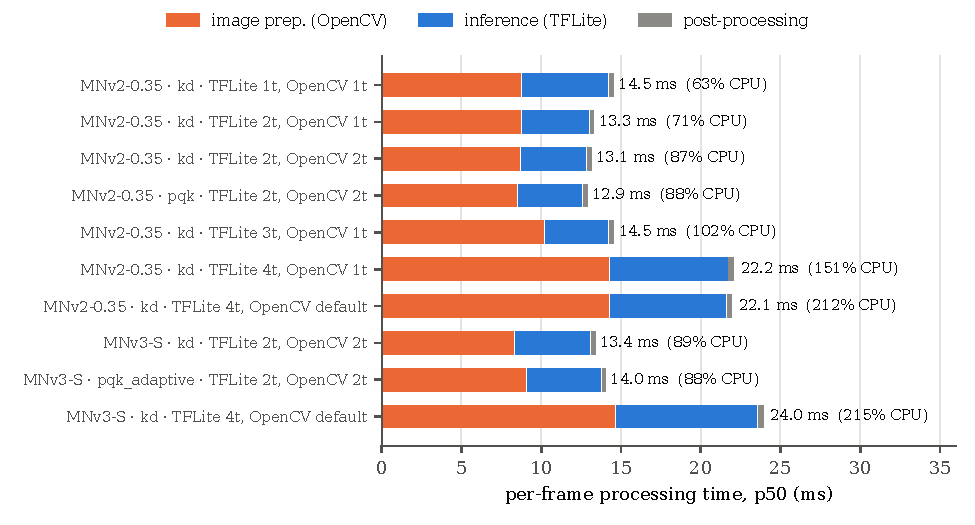
\includegraphics[width=\textwidth]{camera_pipeline}
  \caption{Median per-frame processing time of the live camera pipeline ($640{\times}480$ MJPEG) on the Raspberry Pi~4B, split into image preparation, inference and post-processing, with the process CPU use, for different thread counts.}
  \label{fig:camera}
\end{figure*}

\begin{table*}[t]
  \centering
  \caption{Live camera pipeline: median time per stage (ms), achieved frame rate and process CPU use, by number of TFLite and OpenCV threads (``default'' lets OpenCV use all cores).}
  \label{tab:camera}
  \adjustbox{max width=\textwidth}{\begin{tabular}{@{}llrrrrrrrrr@{}}
\toprule
Student & Method & TFLite thr. & CV thr. & preproc. & invoke & post & processing & FPS & CPU \% & max $^\circ$C \\
\midrule
MobileNetV2-0.35 & \texttt{kd} & 1 & 1 & 8.8 & 5.5 & 0.24 & 14.2 & 30.0 & 63 & 50.1 \\
MobileNetV2-0.35 & \texttt{kd} & 2 & 1 & 8.8 & 4.3 & 0.24 & 12.9 & 30.0 & 71 & 50.1 \\
MobileNetV2-0.35 & \texttt{kd} & 2 & 2 & 8.8 & 4.1 & 0.24 & 12.8 & 30.0 & 87 & 50.1 \\
MobileNetV2-0.35 & \texttt{kd} & 3 & 1 & 10.3 & 4.0 & 0.27 & 13.6 & 30.0 & 102 & 49.2 \\
MobileNetV2-0.35 & \texttt{kd} & 4 & 1 & 14.3 & 7.4 & 0.43 & 22.5 & 29.6 & 151 & 49.2 \\
MobileNetV2-0.35 & \texttt{kd} & 4 & 4 & 14.3 & 7.3 & 0.43 & 22.0 & 29.6 & 212 & 50.1 \\
MobileNetV2-0.35 & \texttt{pqk} & 2 & 2 & 8.6 & 4.1 & 0.24 & 12.6 & 30.0 & 88 & 49.7 \\
MobileNetV3-S & \texttt{kd} & 2 & 2 & 8.4 & 4.8 & 0.22 & 13.3 & 30.0 & 89 & 50.6 \\
MobileNetV3-S & \texttt{kd} & 4 & 4 & 14.7 & 8.9 & 0.42 & 24.1 & 28.6 & 215 & 49.2 \\
MobileNetV3-S & \texttt{pqk\_adaptive} & 2 & 2 & 9.1 & 4.7 & 0.22 & 13.5 & 30.0 & 88 & 50.1 \\
\bottomrule
\end{tabular}
}
\end{table*}

The webcam delivers about $30$ frames per second, so the pipeline is bounded by the camera whenever the processing time is below $33$\,ms.
With one to three inference threads every configuration reaches $29.99$ frames per second. The best one, two TFLite and two OpenCV threads, takes $12.8$\,ms of processing at $87\%$ CPU use.
Giving the inference all four cores raises the processing time by a factor of $1.7$ to $1.8$ ($22.0$ to $22.5$\,ms for MobileNetV2-0.35 and $24.1$\,ms for MobileNetV3-Small, against $12.8$ and $13.3$\,ms), at $150\%$ to $215\%$ CPU use. Image preparation itself slows from $8.8$ to $14.3$\,ms, and one OpenCV thread is as slow as the default.
MobileNetV3-Small then falls slightly below the camera rate ($28.6$ frames per second). We did not investigate the cause.
Image preparation ($8.8$\,ms) costs more than inference ($4.1$\,ms).
The frames come from an unconstrained scene, so the predicted classes are a demonstration, not a measurement.

\begin{figure*}[t]
  \centering
  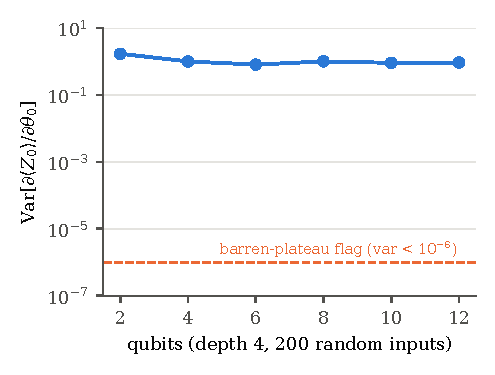
\includegraphics[width=0.55\textwidth]{barren_plateau}
  \caption{Variance of the derivative of $\langle Z_0\rangle$ with respect to the first input angle over $200$ random inputs, as a function of the number of qubits (depth $4$).}
  \label{fig:barren}
\end{figure*}

We checked that the circuit does not enter a barren-plateau regime at the width used (Figure~\ref{fig:barren}).
The gradient variance stays between $0.8$ and $1.7$ from $2$ to $12$ qubits, with no exponential decay, as expected for a shallow circuit with a local observable.
The circuit has no trainable parameters, so this concerns the gradient with respect to the input angles that reach the student.

\section{Recipe Audit}
\label{app:recipe}

Within each pair, all runs share one training recipe (epoch budget, patience, optimizer, learning rate, weight decay, batch size and BatchNorm handling), and within each cell all seeds share the loss settings.
Auditing the stored recipes found two exceptions, both on RPS-25/LeNet-5.

\paragraph{A \Scratch seed with a different budget (Table~\ref{tab:rule3}).}
Seed~0 of \Scratch on RPS-25/LeNet-5 was trained with a budget of $40$ epochs and patience $8$. The other seeds of that pair and all other methods used $60$ and $12$.
It ran all $40$ epochs, so it was limited by its budget and not stopped early. Its score is the lowest of the three.
We did not re-run it.
Excluding it makes \Scratch stronger on that pair ($0.736\pm0.044$ over the two matched seeds, against $0.676\pm0.108$ as reported), and \Pqk $-$ \Scratch goes from $-0.039$ to $-0.060$. The conclusion that \Scratch beats every distillation method there is unchanged.
The variance comparison does change. The pair's \Scratch standard deviation falls from $0.108$ to $0.044$ (two seeds), and the number of pairs on which \Pqk has a lower standard deviation than \Scratch falls from \VarBelowScratch{} to \VarBelowScratchEx{} of \NPairs{}.
Comparisons of \Pqk with \Rbf and with \Kd do not involve \Scratch and are unaffected by this run.

\paragraph{A \Kd cell with two temperatures.}
The \Kd cell for this pair mixes two settings. Seed~0 was trained at $\tau=0.5$, the temperature of the kernel methods. Seeds~1 and~2 were trained at $\tau=1$, in an earlier run at which the temperature was screened, and only seed~0 was repeated at the final value.
The three scores are $0.639$, $0.663$ and $0.649$, so the cell mean of $0.650\pm0.012$ in Table~\ref{tab:main} combines the two.
Using only the two seeds at the majority temperature, \Kd scores $0.656\pm0.010$, and \Pqk $-$ \Kd on this pair goes from $-0.013$ (as reported) to $+0.021$. On seed~0 alone it is $-0.080$.
The pair therefore flips sign depending on the seeds used. The number of pairs on which \Pqk is ahead of \Kd at fp32 is \KdAheadFp{} as reported and \KdAheadFpEx{} without seed~0.
The \Kd standard deviation for the pair, which is the lowest of any method in Table~\ref{tab:var}, mixes the two temperatures as well.
We did not re-run the two seeds, because that would require replacing stored results. The conclusion that \Pqk and \Kd are indistinguishable is unaffected, and both counts are given in the text.

\begin{table*}[t]
  \centering
  \caption{The recipe audit. $^{\S}$Run trained with a different budget and patience from the rest of its pair.}
  \label{tab:rule3}
  \adjustbox{max width=0.85\textwidth}{\begin{tabular}{@{}llrrrr@{}}
\toprule
Run & Seed & Budget & Patience & Epochs run & Macro-F1 \\
\midrule
RPS-25/LeNet-5, \texttt{scratch} & 0$^{\S}$ & 40 & 8 & 40 & $0.556$ \\
RPS-25/LeNet-5, \texttt{scratch} & 1 & 60 & 12 & 39 & $0.705$ \\
RPS-25/LeNet-5, \texttt{scratch} & 2 & 60 & 12 & 46 & $0.767$ \\
\midrule
all three seeds (as reported) & & & & & $0.676\pm0.108$ \\
matched seeds only ($n=2$) & & & & & $0.736\pm0.044$ \\
\bottomrule
\end{tabular}
}
\end{table*}

\section{Alignment of the Teacher Kernel with the Labels}
\label{app:ckta}

Table~\ref{tab:ckta} gives the centered kernel--target alignment (CKTA) between each target kernel and the label kernel $YY^{\top}$. A value of $1$ means the kernel encodes the class partition exactly.
Each target is the RBF kernel (median heuristic) of the feature map named in the row, applied to the teacher's features after the projection named in the first column.
Random projections are averaged over five draws, and fitted projections use the training split only.
The validation columns use the whole validation split. The training-batch columns use $50$ random batches of $128$ training images, which is where the loss is computed. They are computed from the teacher's features of the unaugmented training images, so they approximate the augmented batches seen in training.
The test split is never used.

\begin{table*}[t]
  \centering
  \caption{Centered kernel--target alignment of the teacher kernel with the label kernel, on validation and on $128$-image training batches.}
  \label{tab:ckta}
  \adjustbox{max width=\textwidth}{\begin{tabular}{@{}llcccc@{}}
\toprule
 & & \multicolumn{2}{c}{TrashNet} & \multicolumn{2}{c}{RPS-25} \\
\cmidrule(lr){3-4}\cmidrule(lr){5-6}
Projection & Target kernel & val. & train batches & val. & train batches \\
\midrule
-- & raw teacher 2048-d, RBF & $0.720$ & $0.818$ & $0.864$ & $0.936$ \\
\midrule
random (fixed) & angles, RBF & $0.363$ & $0.447$ & $0.684$ & $0.765$ \\
 & PQK (RY+CNOT), 16 coords & $0.245$ & $0.297$ & $0.539$ & $0.617$ \\
 & no-CNOT, 16 coords & $0.323$ & $0.408$ & $0.641$ & $0.703$ \\
\midrule
PCA (fitted) & angles, RBF & $0.666$ & $0.793$ & $0.783$ & $0.615$ \\
 & PQK (RY+CNOT), 16 coords & $0.531$ & $0.672$ & $0.754$ & $0.583$ \\
 & no-CNOT, 16 coords & $0.494$ & $0.636$ & $0.587$ & $0.480$ \\
\midrule
LDA+PCA (fitted) & angles, RBF & $0.825$ & $0.963$ & $0.861$ & $0.844$ \\
 & PQK (RY+CNOT), 16 coords & $0.752$ & $0.902$ & $0.797$ & $0.897$ \\
 & no-CNOT, 16 coords & $0.676$ & $0.855$ & $0.636$ & $0.659$ \\
\bottomrule
\end{tabular}
}
\end{table*}
